\subsection{Clean Architecture}
\gls{ca} is a software design approach emphasizing code organization into independent,
modular layers with distinct responsibilities. This approach aims to create a more
flexible, maintainable, and testable software system by enforcing the separation of
concerns and minimizing dependencies between components. \gls{ca} aims to provide a solid
foundation for software development, allowing developers to build applications that can
adapt to changing requirements, scale effectively, and remain resilient against the
introduction of bugs \parencite{r_c_martin_clean_2018}.

\gls{ca} organizes its components into distinct layers. This architecture promotes the
separation of concerns, maintainability, testability, and adaptability. The following list
briefly describes each layer \parencite{r_c_martin_clean_2018}. By organizing code into
these layers and adhering to the principles of \gls{ca}, developers can create more
flexible, maintainable, and testable software with well-defined boundaries and a
separation of concerns.

\begin{itemize} \label{list:layers}
    \item \highlight{Domain Layer}: This layer contains the application's core business
    objects, rules, and domain logic. Entities represent the fundamental concepts and
    relationships in the problem domain and are independent of any specific technology
    or framework. The domain layer focuses on encapsulating the essential complexity of
    the system and should be kept as pure as possible.
    \item \highlight{Application Layer}: This layer contains the use cases or
    application-specific business rules orchestrating the interaction between entities and
    external systems. Use cases define the application's behavior regarding the actions
    users can perform and the expected outcomes. This layer coordinates the data flow
    between the domain layer and the presentation or infrastructure layers while remaining
    agnostic to the specifics of the user interface or external dependencies.
    \item \highlight{Presentation Layer}: This layer translates data and interactions
    between the use cases and external actors, such as users or external systems.
    Interface adapters include controllers, view models, presenters, and data mappers,
    which handle user input, format data for display, and convert data between internal
    and external representations. The presentation layer should be as thin as possible,
    focusing on the mechanics of user interaction and deferring application logic to the
    use cases.
    \item \highlight{Infrastructure Layer}: This layer contains the technical
    implementations of external systems and dependencies, such as databases, web services,
    file systems, or third party libraries. The infrastructure layer provides concrete
    implementations of the interfaces and abstractions defined in the other layers,
    allowing the core application to remain decoupled from specific technologies or
    frameworks. This layer is also responsible for configuration or initialization code to
    set up the system's runtime environment.
\end{itemize}

\begin{figure}[H]
    \centering
    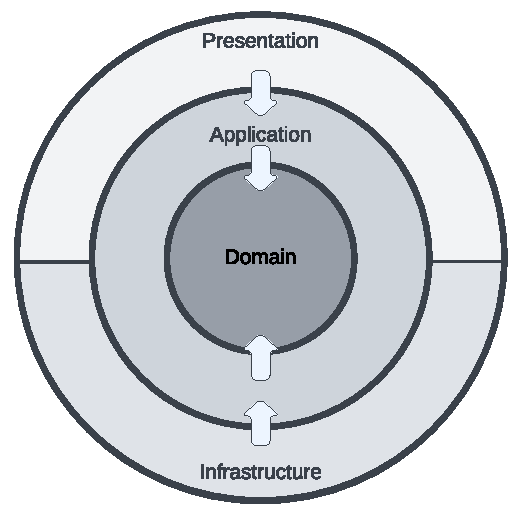
\includegraphics[width=0.3\textwidth]{figures/ca_diagram.pdf}
    \caption[Flow of control]{Flow of control}
    \label{fig_modulair_components}
\end{figure}

An essential aspect is described as the dependency rule. The rule states that
\textit{source code dependencies must point only inward toward higher-level policies}
(Robert C. Martin, 2018, p. 206). This ’flow of control’ is designed following the
\gls{dip} and can be represented schematically as concentric circles containing all the
described components. The arrows in Figure \ref{fig_modulair_components} clearly show that
the dependencies flow from the outer layers to the inner layers. Most outer layers are
historically subjected to large-scale refactorings due to technological changes and
innovation. Separating the layers and adhering to the dependency rule ensures that the
domain logic can evolve independently from external dependencies or certain specific
technologies.

\textcite[78]{r_c_martin_clean_2018} argues that software can quickly become a
well-intended mess of bricks and building blocks without rigorous design principles. So,
from the early 1980s, he began to assemble a set of software design principles as
guidelines to create software structures that tolerate change and are easy to understand.
The principles are intended to promote modular and component-level software structure
\parencite[79]{r_c_martin_clean_2018}. In 2004, the principles were established to form
the acronym SOLID. 

The following list will provide an overview of each of the SOLID principles.

\begin{itemize}
    \item \glslong{srp}: This principle has undergone several iterations of the formal
    definition. The final definition of the Single Responsibility Principle (SRP) is:
    \enquote{a module should be responsible to one, and only one, actor}
    \textcite[82]{r_c_martin_clean_2018}. The word \enquote*{actor} in this statement refers to all
    the users and stakeholders represented by the (functional) requirements. The
    modularity concept in this definition is described by
    \textcite[82]{r_c_martin_clean_2018} as a cohesive set of functions and data
    structures. In conclusion, this principle allows for modules with multiple tasks as
    long as they cohesively belong together. \textcite[81]{r_c_martin_clean_2018}
    acknowledges the slightly inappropriate name of the principle, as many interpreted it,
    that a module should do just one thing.
    \item \glslong{ocp}: \textcite{meyer_object-oriented_1988} first mentioned the
    \gls{ocp} and formulated the following definition: \textit{A module should be open for
    extension but closed for modification.} The software architecture should be designed
    such that the behavior of a module can be extended without modifying existing source
    code. The \gls{ocp} promotes the use of abstraction and polymorphism to achieve this
    goal. The \gls{ocp} is one of the driving forces behind the software architecture of
    systems, making it relatively easy to apply new requirements.
    \parencite[94]{r_c_martin_clean_2018}.
    \item \glslong{lsp}: The \gls{lsp} is named after Barbara Liskov, who first introduced
    the principle in a paper she co-authored in 1987. Barbara Liskov wrote the following
    statement to define subtypes (Robert C. Martin, 2018, p. 95). \textit{If for each
    object o1 of type S, there is an object o2 of type T such that for all programs P
    defined in terms of T, the behavior of P is unchanged when o1 is substituted for o2
    then S is a subtype of T.1.} Or in simpler terms: To build software from
    interchangeable parts, those parts must adhere to a contract that allows those parts
    to be substituted for another (Robert C. Martin, 2018, p. 80)
    \item \glslong{isp}: The \gls{isp} suggests that software components should have
    narrow, specific interfaces rather than broad, general-purpose ones. In addition, the
    \gls{isp} states that consumer code should not be allowed to depend on methods it does
    not use. In other words, interfaces should be designed to be as small and focused as
    possible, containing only the methods relevant to the consumer code using them. This
    allows the consumer code to use only the needed methods without being forced to
    implement or depend on unnecessary methods
    \parencite[104]{r_c_martin_clean_2018}. 
    \item \glslong{dip}: The \gls{dip} prescribes that high-level modules should not
    depend on low-level modules, and both should depend on abstractions. The principle
    emphasizes that the architecture should be designed so that the flow of control
    between the different objects, layers, and components is always from higher-level
    implementations to lower-level details. In other words, high-level implementations,
    like business rules, should not be concerned about low-level implementations, such as
    how the data is stored or presented to the end user. Additionally, high-level and
    low-level implementations should only depend on abstractions or interfaces defining a
    contract for how they should interact \parencite[91]{r_c_martin_clean_2018}. This
    approach allows for great flexibility and a modular architecture. Modifications in the
    low-level implementations will not affect the high-level implementations as long as
    they still adhere to the contract defined by the abstractions and interfaces.
    Similarly, changes to the high-level modules will not affect the low-level modules as
    long as they still fulfill the contract. This reduces coupling and ensures the
    evolvability of the system over time, as changes can be made to specific modules
    without affecting the rest of the system.
\end{itemize}

\textcite{r_c_martin_clean_2018} proposes the following elements to achieve
the goal of \enquote{Clean Architecture.}

\begin{itemize}
    \item \highlight{Entities}: Entities are the core business objects, representing the
    domain's fundamental data.
    \item \highlight{Interactor}: Interactors encapsulate business logic and represent
    specific actions that the system can perform.
    \item \highlight{RequestModels}: RequestModels represent the input data required by a
    specific interactor.
    \item \highlight{ResponseModel}: ResponseModel represents the output data
    required by a specific interactor.
    \item \highlight{ViewModels}: ViewModels are responsible for managing the data and
    behavior of the user interface.
    \item \highlight{Controllers}: Controllers are responsible for handling requests from the user
    interface and routing them to the appropriate Interactor.
    \item \highlight{Presenters}: Presenters are responsible for formatting and the data for
    the user interface.
    \item \highlight{Gateways}: A Gateway provides an abstraction layer between the
    application and its external dependencies, such as databases, web services, or other
    external systems.
    \item \highlight{Boundary}: Boundaries are used to separate the different layers of
    the component.
\end{itemize}